\documentclass[11pt,a4paper]{article}
\usepackage[T1]{fontenc}
\usepackage[utf8]{inputenc}
\usepackage{lmodern}
\usepackage{amsmath,amssymb}
\usepackage{graphicx}
\usepackage{booktabs}
\usepackage{tikz}
\usepackage{hyperref}
\hypersetup{colorlinks=true,linkcolor=blue!60!black,citecolor=blue!60!black,urlcolor=blue!60!black}
\usetikzlibrary{positioning,calc}
\usepackage{microtype}
\usepackage{geometry}
\usepackage{authblk}
\usepackage{multicol}
\geometry{margin=2.7cm}

\title{Motzkin Neighborhood for Permutation Flow Shop}

\author[1]{Remigiusz Wojewódzki}
\author[2]{Wojciech Bożejko}
\affil[1]{Wrocław University of Science and Technology}
\affil[2]{Wrocław University of Science and Technology}
\date{November 2025}

\begin{document}
\maketitle

\begin{abstract}
We introduce a new neighborhood for the permutation Flow Shop Problem in which a move consists of multiple nested endpoint swaps of segments. Admissible configurations correspond to structures enumerated by the Motzkin numbers $M_n$. We describe a dynamic programming algorithm with complexity $O(mn^3)$ for selecting the optimal set of swaps and analyze the combinatorial properties of the move space. The neighborhood enables exploration of deeper permutation structures in metaheuristics such as Tabu Search and Simulated Annealing.
\end{abstract}

\section{Introduction}

The permutation Flow Shop Problem consists of finding a permutation of $n$ jobs executed on $m$ machines in the same order, minimizing the completion time (makespan) $C_{\max}$. Classical neighborhoods (e.g., adjacent swap) explore the space locally and shallowly. The motivation for this work is to construct a richer composite move that preserves a structure enabling efficient optimization while encompassing multiple coordinated swaps.

\section{Characterization of Motzkin Numbers}

Motzkin numbers $M_n$ enumerate \emph{planar} (non-crossing) structures over a set of $n$ ordered points, where each point can be (i) the beginning of an arc, (ii) the end of an arc, or (iii) isolated. They constitute a generalization of Catalan numbers—while the latter require full pairing, Motzkin numbers allow singleton points.

\paragraph{Equivalent representations.}
Motzkin objects can be interpreted as:
\begin{enumerate}
  \item Lattice paths with steps $(1,+1)$, $(1,0)$, $(1,-1)$ not descending below the axis $y=0$.
  \item Non-crossing families of arcs over a line with optional isolated points.
  \item Enriched triangulations or dissections of polygons.
\end{enumerate}
In our neighborhood, each permutation index can participate as a left endpoint of an arc, a right endpoint of an arc, or remain untouched—precisely three states corresponding to the Motzkin structure.

\paragraph{Recurrences.}
The basic convolution recurrence follows from decomposing the first point:
\begin{align*}
M_0 &= 1,\quad M_1 = 1,\\
M_n &= M_{n-1} + \sum_{k=0}^{n-2} M_k\, M_{n-2-k}\quad (n \ge 2).
\end{align*}
Interpretation: if point 0 is isolated, there remain $M_{n-1}$ configurations; if it opens an arc closed at point $k+1$, the interior (points $1\ldots k$) and the outer tail (points $k+2\ldots n-1$) are independent, yielding the product $M_k M_{n-2-k}$.

Alternative linear recurrence:
\[
M_n = \frac{(2n+1)M_{n-1} + 3(n-1)M_{n-2}}{n+2},\quad n \ge 2.
\]

Generating function:
\[
M(x) = \sum_{n\ge0} M_n x^n = \frac{1 - x - \sqrt{1 - 2x - 3x^2}}{2x^2}.
\]

\paragraph{Asymptotics}
Asymptotically $M_n \sim c\,3^n / n^{3/2}$ for the constant $c = \frac{3\sqrt{3}}{2\sqrt{\pi}}$. The space of admissible composite moves grows significantly slower than $2^{\binom{n}{2}}$ (the set of all subsets of index pairs), making full dynamic programming practical.

\begin{table}[ht]
  \centering
  \caption{First Motzkin numbers ($n=0..10$).}
  \begin{tabular}{@{}rcccccccccccc@{}}
    \toprule
    $n$ & 0 & 1 & 2 & 3 & 4 & 5 & 6 & 7 & 8 & 9 & 10 \\
    \midrule
    $M_n$ & 1 & 1 & 2 & 4 & 9 & 21 & 51 & 127 & 323 & 835 & 2188 \\
    \bottomrule
  \end{tabular}
\end{table}

\paragraph{Example: computing $M_4$.}
Applying the convolution recurrence:
\[
\begin{aligned}
M_2 &= M_1 + M_0 M_0 = 1 + 1 = 2, \\
M_3 &= M_2 + (M_0 M_1 + M_1 M_0) = 2 + 2 = 4, \\
M_4 &= M_3 + (M_0 M_2 + M_1 M_1 + M_2 M_0) = 4 + (2 + 1 + 2) = 9.
\end{aligned}
\]

\medskip
Having established the combinatorial foundations of Motzkin numbers, we now proceed to the construction of the neighborhood for the permutation Flow Shop.

\section{Structure of the Motzkin Neighborhood}

The proposed neighborhood represents a transition from classical single-parameter moves (e.g., a single adjacent swap) to \emph{structurally composite} multi-moves that can transform a permutation in one step through several coordinated local modifications—similar to Dynasearch or the Fibonacci neighborhood.

The guiding idea is to limit the combinatorial explosion by imposing a strict, easily verifiable structure: each index pair $(i,j)$ describes an endpoint swap of a segment, and a set of such pairs is admissible only when the corresponding arcs (interpreted as connections $i \to j$ over the index line) are \emph{non-crossing}, may \emph{nest}, but do not share endpoints. In this way, in one iteration we search a larger horizon of potential solutions while maintaining complexity control.

\subsection{Move Definition and Admissibility Conditions}

\paragraph{Endpoint swap.}
For a permutation $\pi = (\pi_0,\pi_1,\ldots,\pi_{n-1})$ and an index pair $(i,j)$ satisfying $0 \le i < j < n$, we define an \emph{endpoint swap} as the operation:
\[
S_{i,j}(\pi) = (\pi_0,\ldots,\pi_{i-1},\; \pi_j,\; \pi_{i+1},\ldots,\pi_{j-1},\; \pi_i,\; \pi_{j+1},\ldots,\pi_{n-1}).
\]
This operation swaps the elements at positions $i$ and $j$, preserving the order of all intermediate elements $\pi_{i+1},\ldots,\pi_{j-1}$. Locally, the segment $[\pi_i,\pi_{i+1},\ldots,\pi_{j-1},\pi_j]$ transforms into $[\pi_j,\pi_{i+1},\ldots,\pi_{j-1},\pi_i]$.

\paragraph{Composite move: set of concurrent swaps.}
A \emph{composite move} is a set $\mathcal{M} = \{(i_1,j_1), (i_2,j_2), \ldots, (i_k,j_k)\}$ of index pairs. The set $\mathcal{M}$ is \emph{admissible} if it satisfies the following conditions:

\begin{enumerate}
  \item \textbf{Endpoint disjointness}: For any two pairs $(i_a,j_a), (i_b,j_b) \in \mathcal{M}$, we have $\{i_a,j_a\} \cap \{i_b,j_b\} = \varnothing$ (no two pairs share an index).
  
  \item \textbf{No crossing}: The pattern $i_a < i_b < j_a < j_b$ is forbidden for any $(i_a,j_a), (i_b,j_b) \in \mathcal{M}$ (arcs cannot intersect).
  
  \item \textbf{Nesting allowed}: The configuration $i_a < i_b < j_b < j_a$ is acceptable (inner pair fully contained within outer pair).
\end{enumerate}

Applying all swaps from the set $\mathcal{M}$ in order of increasing left endpoints $i_k$ yields a unique result—conditions (1)–(3) guarantee that no pair interferes with the effect of another pair. Each pair modifies only two permutation elements at the endpoint positions; the internal segment preserves order, and the simulation of nested arcs proceeds independently.

\begin{figure}[ht]
  \centering
  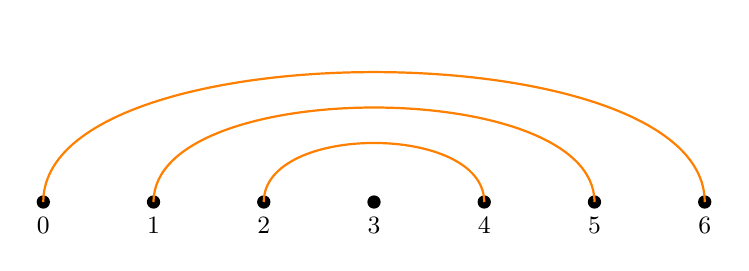
\begin{tikzpicture}[scale=1.0, baseline=(current bounding box.center)]
    \def\N{7}
    \def\DX{1.4}
    \def\Ybase{0}
    \foreach \i in {0,...,6} {
      \coordinate (P\i) at (\i*\DX,\Ybase);
      \fill (P\i) circle (2.4pt);
      \node[below=2pt, font=\small] at (P\i) {\i};
    }
    \draw[orange, thick] (P0) .. controls +(.0,2.2) and +(-.0,2.2) .. (P6);
    \draw[orange, thick] (P1) .. controls +(.0,1.6) and +(-.0,1.6) .. (P5);
    \draw[orange, thick] (P2) .. controls +(.0,1.0) and +(-.0,1.0) .. (P4);
  \end{tikzpicture}
  \caption{Example of an admissible composite move: nested arcs $(0,6)$, $(1,5)$, $(2,4)$; point 3 isolated.}
\end{figure}

\paragraph{Bijection with Motzkin objects.}
The key observation is that the set of admissible composite moves for $n$ indices has cardinality exactly equal to $M_n$ (the Motzkin number). Interpretation: each index $0 \le i < n$ can be in one of three states:
\begin{itemize}
  \item \textbf{Left endpoint of an arc}: there exists a pair $(i,j) \in \mathcal{M}$.
  \item \textbf{Right endpoint of an arc}: there exists a pair $(k,i) \in \mathcal{M}$.
  \item \textbf{Isolated}: the index participates in no pair.
\end{itemize}
This three-state property corresponds exactly to the definition of Motzkin objects (paths with steps $+1$, $0$, $-1$ or families of arcs with isolated points). Conditions (1)–(3) encode non-crossing and disjointness, which is the essence of the Motzkin structure.

\paragraph{Space size and algorithmic implications.}
The space of admissible composite moves has size $M_n \sim c \cdot 3^n / n^{3/2}$, which is significantly smaller than $2^{\binom{n}{2}}$ (all subsets of index pairs). This controlled space size justifies the use of full dynamic programming to select the optimal composite move—in contrast to naive searching of an exponential number of combinations, the DP algorithm operates on $O(n^2)$ states, considering $O(n)$ candidates per state.

\section{Algorithm for Selecting the Optimal Composite Move}

Having defined the space of admissible composite moves, we need an algorithm that in polynomial time selects a set of pairs $\mathcal{M}$ minimizing the makespan. The algorithm consists of five steps:
\begin{enumerate}
  \item Computing prefix completion columns $F[k][r]$ (preprocessing).
  \item Enumerating deltas $\Delta_{i,j}$ for all pairs $(i,j)$.
  \item Dynamic programming: filling the table $\mathrm{dp}[L][R]$.
  \item Reconstructing the selected set of pairs $\mathcal{M}$.
  \item Applying the swaps to permutation $\pi$.
\end{enumerate}

\subsection{Computing deltas}

For each index pair $(i,j)$ with $0 \le i < j < n$ we compute the makespan change:
\[
\Delta_{i,j} = C_{\max}(S_{i,j}(\pi)) - C_{\max}(\pi).
\]
where:
\begin{itemize}
  \item $\Delta_{i,j}$ — change in makespan after swapping positions $i$ and $j$
  \item $S_{i,j}(\pi)$ — permutation after endpoint swap operation on indices $(i,j)$
  \item $C_{\max}(\cdot)$ — makespan (completion time on last machine for all jobs)
\end{itemize}

In the implementation we use \emph{prefix completion columns} $F[k][r]$, where $F[k][r]$ denotes the completion time on machine $r$ after processing the first $k$ jobs of permutation $\pi$. We compute these columns using standard DP for FSP:
\[
\begin{aligned}
F[0][r] &= 0 \quad \text{for all } r, \\
F[k][0] &= F[k-1][0] + p_{0,\pi_{k-1}}, \\
F[k][r] &= \max(F[k][r-1], F[k-1][r]) + p_{r,\pi_{k-1}}, \quad r \ge 1,
\end{aligned}
\]
where:
\begin{itemize}
  \item $F[k][r]$ — completion time on machine $r$ after processing first $k$ jobs
  \item $p_{r,j}$ — processing time of job $j$ on machine $r$
  \item $\pi_{k-1}$ — job at position $k-1$ in current permutation
  \item $F[k][r-1]$ — time when machine $r$ finished previous job (waiting for machine)
  \item $F[k-1][r]$ — time when previous job finished on machine $r$ (waiting for job)
  \item $\max(\cdot)$ — machine must wait for both: previous job on same machine AND same job on previous machine
\end{itemize}

Then, for pair $(i,j)$, starting from prefix state $F[i]$, we simulate the new segment order:
\[
[\pi_j, \pi_{i+1}, \ldots, \pi_{j-1}, \pi_i],
\]
and then complete with the tail simulation $\pi_{j+1}, \ldots, \pi_{n-1}$. Cost of a single delta: $O(m(n-i))$. Full enumeration of all $\binom{n}{2}$ pairs: $O(mn^3)$.

\subsection{Dynamic programming recurrence}

We define the function $\mathrm{dp}[L][R]$ as the \emph{minimum sum of deltas} achievable by selecting an admissible set of pairs in the index interval $[L, R]$. 

\paragraph{Notation:}
\begin{itemize}
  \item $\mathrm{dp}[L][R]$ — minimum achievable sum of $\Delta_{i,j}$ values for interval $[L,R]$
  \item $L, R$ — left and right boundaries of the index interval ($0 \le L \le R < n$)
  \item Smaller $\mathrm{dp}[L][R]$ means better improvement (more negative = lower makespan)
\end{itemize}

Boundary conditions:
\[
\mathrm{dp}[L][R] = 0 \quad \text{for } L \ge R.
\]
\emph{Interpretation:} Empty or single-element intervals contribute zero change (no pairs can be formed).

For interval $[L, R]$ with $L < R$ we consider two cases:

\paragraph{Case 1: Skip index $L$}
We do not use $L$ as the left endpoint of any arc:
\[
\text{Value} = \mathrm{dp}[L+1][R]
\]
\emph{Interpretation:} Index $L$ remains isolated; optimal solution comes from subproblem $[L+1, R]$.

\paragraph{Case 2: Select arc $(L, k)$}
For some $k \in \{L+1, \ldots, R\}$, we pair index $L$ with index $k$. The interval splits into:
\begin{itemize}
  \item \textbf{Arc interior:} $[L+1, k-1]$ (if non-empty) with value $\mathrm{dp}[L+1][k-1]$
  \item \textbf{Right tail:} $[k+1, R]$ (if non-empty) with value $\mathrm{dp}[k+1][R]$
\end{itemize}

Combined value:
\[
\text{Value} = \Delta_{L,k} + \mathrm{dp}[L+1][k-1] + \mathrm{dp}[k+1][R]
\]
where:
\begin{itemize}
  \item $\Delta_{L,k}$ — makespan change from swapping positions $L$ and $k$
  \item $\mathrm{dp}[L+1][k-1]$ — optimal solution for indices strictly between $L$ and $k$ (nested inside the arc)
  \item $\mathrm{dp}[k+1][R]$ — optimal solution for indices after $k$ (disjoint from arc $(L,k)$)
\end{itemize}

\paragraph{Full recurrence:}
\[
\mathrm{dp}[L][R] = \min\left\{ 
  \mathrm{dp}[L+1][R], \; 
  \min_{k=L+1}^{R} \big( \Delta_{L,k} + \mathrm{dp}[L+1][k-1] + \mathrm{dp}[k+1][R] \big)
\right\}.
\]

\emph{Interpretation:} We choose the option (skip $L$ or pair it with some $k$) that minimizes the total delta sum.

\paragraph{Computation order:}
We fill the table for increasing interval lengths $\ell = R - L + 1$ from $\ell=2$ to $\ell=n$:
\begin{enumerate}
  \item $\ell = 2$: intervals $[0,1], [1,2], \ldots, [n-2,n-1]$
  \item $\ell = 3$: intervals $[0,2], [1,3], \ldots, [n-3,n-1]$
  \item $\vdots$
  \item $\ell = n$: interval $[0,n-1]$ (entire permutation)
\end{enumerate}

The final value $\mathrm{dp}[0][n-1]$ gives the optimal total delta for the entire permutation.

Although deltas of individual pairs are not strictly additive (makespan depends globally on the entire permutation), the non-crossing structure ensures that local swap effects can be effectively aggregated within the DP algorithm.

\subsection{Reconstructing the selected pair set}

While filling the table $\mathrm{dp}$, we remember for each interval $[L,R]$ the optimal choice in table $\mathrm{choice}[L][R]$:
\[
\mathrm{choice}[L][R] = 
\begin{cases}
\text{None}, & \text{if we skip } L, \\
k, & \text{if we select arc } (L,k).
\end{cases}
\]

Reconstruction proceeds recursively:
\begin{verbatim}
function reconstruct(L, R):
    if L >= R: return
    k = choice[L][R]
    if k == None:
        reconstruct(L+1, R)
    else:
        add pair (L, k) to result
        reconstruct(L+1, k-1)
        reconstruct(k+1, R)
\end{verbatim}

Result: a list of pairs $\mathcal{M} = \{(i_1, j_1), (i_2, j_2), \ldots\}$ satisfying all admissibility conditions (non-crossing, no shared endpoints, allowed nesting).

\subsection{Applying the composite move}

We apply the obtained set of pairs $\mathcal{M}$ to permutation $\pi$ in order of increasing left endpoints:
\[
\text{for each pair } (i,j) \in \mathcal{M} \text{ (sorted by } i\text{)}: \quad \pi[i] \leftrightarrow \pi[j].
\]
Due to the admissibility conditions, the swaps are mutually independent—each index appears in at most one pair.

\subsection{Computational complexity}

\paragraph{Time.}
\begin{itemize}
  \item Preprocessing (prefix columns $F$): $O(mn)$.
  \begin{itemize}
    \item For each of $n$ positions, compute completion times on $m$ machines
  \end{itemize}
  
  \item Enumeration of deltas $\Delta_{i,j}$ for all pairs: $O(mn^3)$.
  \begin{itemize}
    \item $\binom{n}{2} = O(n^2)$ pairs total
    \item Each pair: simulate segment of average length $O(n)$ on $m$ machines
    \item Total: $O(n^2) \times O(mn) = O(mn^3)$
  \end{itemize}
  
  \item Filling the DP table: $O(n^3)$.
  \begin{itemize}
    \item $O(n^2)$ intervals $[L,R]$ to fill
    \item Each interval: test $O(n)$ candidates for $k$
    \item Total: $O(n^2) \times O(n) = O(n^3)$
  \end{itemize}
  
  \item Reconstruction: $O(n)$.
  \begin{itemize}
    \item At most $n/2$ pairs can be selected (each uses 2 indices)
  \end{itemize}
  
  \item Applying swaps: $O(n)$.
  \begin{itemize}
    \item Each of $O(n)$ swaps takes $O(1)$ time
  \end{itemize}
\end{itemize}
Total complexity of one neighborhood iteration: $\mathbf{O(mn^3)}$.

\medskip
\noindent\textbf{Dominant term:} Delta enumeration $O(mn^3)$ dominates for typical FSP instances where $m \ll n$.

\paragraph{Space.}
\begin{itemize}
  \item Delta array $\Delta$: $O(n^2)$.
  \begin{itemize}
    \item Upper triangular matrix: $\binom{n}{2} \approx n^2/2$ entries
  \end{itemize}
  
  \item DP tables ($\mathrm{dp}$, $\mathrm{choice}$): $O(n^2)$.
  \begin{itemize}
    \item Two triangular matrices: $O(n^2)$ entries each
  \end{itemize}
  
  \item Prefix columns $F$: $O(mn)$.
  \begin{itemize}
    \item Store $n+1$ columns, each with $m$ machine times
  \end{itemize}
\end{itemize}
Total: $\mathbf{O(n^2 + mn)}$.

\medskip
\noindent\textbf{Practical note:} For $n \le 200$, space requirements are modest ($< 100$MB for typical instances).

\section{Illustrative Example}

Consider a small FSP instance with $n=5$ jobs and $m=3$ machines. Initial permutation:
\[
\pi = (0, 1, 2, 3, 4).
\]

Processing times (rows = machines, columns = jobs):
\[
P = \begin{bmatrix}
3 & 2 & 5 & 4 & 3 \\
2 & 4 & 3 & 2 & 5 \\
4 & 3 & 2 & 5 & 4
\end{bmatrix}
\]

\paragraph{Step 1: Baseline makespan}

We compute $C_{\max}(\pi)$ using standard DP:
\[
\begin{array}{c|ccccc}
\text{Machine} & J_0 & J_1 & J_2 & J_3 & J_4 \\
\hline
0 & 3 & 5 & 10 & 14 & 17 \\
1 & 5 & 9 & 13 & 16 & 21 \\
2 & 9 & 12 & 15 & 21 & 25
\end{array}
\]
Baseline makespan: $C_{\max}(\pi) = 25$.

\paragraph{Step 2: Prefix columns}

Array $F[k][r]$ (completion time on machine $r$ after $k$ jobs):
\[
F = \begin{bmatrix}
0 & 0 & 0 \\
3 & 5 & 9 \\
5 & 9 & 12 \\
10 & 13 & 15 \\
14 & 16 & 21 \\
17 & 21 & 25
\end{bmatrix}
\]

\paragraph{Step 3: Enumerating deltas}

For each pair $(i,j)$ we simulate endpoint swap and compute $\Delta_{i,j} = C_{\max}(S_{i,j}(\pi)) - 25$.


\paragraph{Example: pair $(1,3)$.}
New segment order: $[\pi_3, \pi_2, \pi_1] = [3, 2, 1]$.
Starting from $F[1] = (3, 5, 9)$ we simulate:
\begin{itemize}
  \item Job 3: column $(3+4, \max(7,5)+2, \max(9,7)+5) = (7, 9, 14)$
  \item Job 2: column $(7+5, \max(12,9)+3, \max(15,12)+2) = (12, 15, 17)$
  \item Job 1: column $(12+2, \max(14,15)+4, \max(19,14)+3) = (14, 19, 22)$
  \item Job 4 (tail): column $(14+3, \max(17,19)+5, \max(24,17)+4) = (17, 24, 28)$
\end{itemize}
New makespan: $C_{\max}(S_{1,3}(\pi)) = 28$, so $\Delta_{1,3} = 28 - 25 = +3$ (worsening).

\paragraph{Example: pair $(0,4)$.}
New order: $[4, 1, 2, 3, 0]$.
Starting from $F[0] = (0, 0, 0)$ we simulate the entire sequence:
\begin{itemize}
  \item Job 4: $(3, 5, 9)$
  \item Job 1: $(5, 9, 12)$
  \item Job 2: $(10, 13, 15)$
  \item Job 3: $(14, 16, 21)$
  \item Job 0: $(17, 19, 25)$
\end{itemize}
New makespan: $C_{\max} = 25$, so $\Delta_{0,4} = 0$ (no change).

Assume that after full enumeration we obtain:
\[
\Delta = \begin{bmatrix}
 & 0 & +2 & -1 & 0 \\
  & & +1 & +3 & -2 \\
  & & & +2 & -3 \\
  & & & & +1 \\
  & & & &
\end{bmatrix}
\]
(upper triangular part only).

\paragraph{Step 4: Dynamic programming}

\paragraph{Step 4: Dynamic programming}

We fill the table $\mathrm{dp}[L][R]$ for intervals of increasing length.

\paragraph{Length 2:}
For each adjacent pair of indices, we decide: create arc or skip?

\begin{align*}
\mathrm{dp}[0][1] &= \min\{\underbrace{\mathrm{dp}[1][1]}_{\text{skip 0}}, \; \underbrace{\Delta_{0,1}}_{\text{arc (0,1)}} + \underbrace{\mathrm{dp}[1][0]}_{\text{empty}}\} \\
&= \min\{0, \; 0 + 0\} = 0, \quad \mathrm{choice}[0][1] = 1, \\
\\
\mathrm{dp}[1][2] &= \min\{0, \; +1\} = 0, \quad \mathrm{choice}[1][2] = \text{None}, \\
\mathrm{dp}[2][3] &= \min\{0, \; +2\} = 0, \quad \mathrm{choice}[2][3] = \text{None}, \\
\mathrm{dp}[3][4] &= \min\{0, \; +1\} = 0, \quad \mathrm{choice}[3][4] = \text{None}.
\end{align*}

\emph{Interpretation:} Arc $(0,1)$ gives no improvement ($\Delta_{0,1}=0$), but other arcs would worsen the makespan, so we skip them.

\paragraph{Length 3:}
\begin{align*}
\mathrm{dp}[0][2] &= \min\{\underbrace{\mathrm{dp}[1][2]}_{\text{skip 0}}, \; \underbrace{\Delta_{0,1}}_{\text{arc (0,1)}} + \underbrace{\mathrm{dp}[2][2]}_{\text{empty}}, \; \underbrace{\Delta_{0,2}}_{\text{arc (0,2)}} + \underbrace{\mathrm{dp}[1][1]}_{\text{empty}}\} \\
&= \min\{0, \; 0 + 0, \; 2 + 0\} = 0, \quad \mathrm{choice}[0][2] = \text{None}, \\
\\
\mathrm{dp}[1][3] &= \min\{0, \; 1 + 0, \; 3 + 0\} = 0, \quad \mathrm{choice}[1][3] = \text{None}, \\
\\
\mathrm{dp}[2][4] &= \min\{\underbrace{0}_{\text{skip 2}}, \; \underbrace{2}_{\text{arc (2,3)}}, \; \underbrace{-3}_{\text{arc (2,4)}}\} = -3, \quad \mathrm{choice}[2][4] = 4.
\end{align*}

\emph{Key observation:} Arc $(2,4)$ with $\Delta_{2,4} = -3$ gives significant improvement!

\paragraph{Length 4:}
\begin{align*}
\mathrm{dp}[0][3] &= \min\{\mathrm{dp}[1][3], \; \Delta_{0,1} + \mathrm{dp}[2][3], \; \Delta_{0,2} + \mathrm{dp}[1][2], \; \Delta_{0,3} + \mathrm{dp}[1][2]\} \\
&= \min\{0, \; 0 + 0, \; 2 + 0, \; -1 + 0\} = -1, \quad \mathrm{choice}[0][3] = 3, \\
\\
\mathrm{dp}[1][4] &= \min\{\underbrace{\mathrm{dp}[2][4]}_{\text{skip 1} = -3}, \; 1 + 0, \; 3 + 0, \; -2 + 0\} = -3, \quad \mathrm{choice}[1][4] = \text{None}.
\end{align*}

\emph{Interpretation:} For $[1,4]$, best is to skip index 1 and use the solution from $[2,4]$ (which has arc $(2,4)$).

\paragraph{Length 5:}
\begin{align*}
\mathrm{dp}[0][4] &= \min\Big\{\underbrace{\mathrm{dp}[1][4]}_{\text{skip 0}}, \; \underbrace{\Delta_{0,1} + \mathrm{dp}[2][4]}_{\text{arc (0,1) + rest}}, \; \Delta_{0,2} + \mathrm{dp}[1][3], \\
& \qquad \underbrace{\Delta_{0,3} + \mathrm{dp}[1][2] + \mathrm{dp}[4][4]}_{\text{arc (0,3) + interior + tail}}, \; \Delta_{0,4} + \mathrm{dp}[1][3]\Big\} \\
&= \min\{-3, \; 0 + (-3), \; 2 + 0, \; -1 + 0 + 0, \; 0 + 0\} = -3, \\
& \mathrm{choice}[0][4] = \text{None (skip 0)}.
\end{align*}

\emph{Final result:} $\mathrm{dp}[0][4] = -3$ means we can reduce makespan by 3 units.

\emph{Why skip 0?} Both "skip 0" and "arc $(0,1)$ + rest" give $-3$, but the algorithm chooses to skip (simpler structure).

Final value: $\mathrm{dp}[0][4] = -3$ (possible makespan reduction by 3).

\paragraph{Step 5: Reconstruction}

Starting from $[0,4]$:
\begin{enumerate}
  \item $\mathrm{choice}[0][4] = \text{None}$ → skip 0, recursion for $[1,4]$.
  \item $\mathrm{choice}[1][4] = \text{None}$ → skip 1, recursion for $[2,4]$.
  \item $\mathrm{choice}[2][4] = 4$ → select pair $(2,4)$, recursion for $[3,3]$ and $[5,4]$ (empty).
\end{enumerate}
Selected set: $\mathcal{M} = \{(2,4)\}$.

\medskip
\noindent\textbf{Reconstruction trace visualization:}
\[
\begin{array}{rcl}
[0,4] & \xrightarrow{\text{skip 0}} & [1,4] \\
{[1,4]} & \xrightarrow{\text{skip 1}} & [2,4] \\
{[2,4]} & \xrightarrow{\text{select (2,4)}} & \text{Done: } \mathcal{M} = \{(2,4)\}
\end{array}
\]

\emph{Interpretation:} Indices 0 and 1 remain isolated (not swapped), while indices 2 and 4 form an arc (will be swapped).

\paragraph{Step 6: Application}

We swap $\pi[2] \leftrightarrow \pi[4]$:
\[
\pi' = (0, 1, 4, 3, 2).
\]

We calculate the new makespan:
\[
C_{\max}(\pi') = 25 - 3 = 22.
\]

\paragraph{Summary of the example}

The DP algorithm selected the optimal pair $(2,4)$ among all $\binom{5}{2} = 10$ possible pairs and their combinations, achieving a makespan reduction of 3 units with complexity $O(mn^3) = O(3 \cdot 125) = O(375)$ basic operations.



\section{Comparison with Classical Neighborhoods}
\begin{itemize}
  \item \textbf{Adjacent swap}: extremely cheap ($O(mn)$ per move), but shallow — requires many steps to reach a permutation accessible by a single Motzkin move. High number of iterations per unit time, but limited exploration of the space.
  
  \item \textbf{Fibonacci neighborhood (composite disjoint)}: allows collecting several disjoint swaps in one step, but without nesting of arcs. The Motzkin neighborhood extends this idea with a full hierarchy of nested structures, increasing the richness of a single move.
  
  \item \textbf{Dynasearch}: explores sequences of structural moves (often 2-exchange in different segments), but its space is not based on a coherent combinatorial object. It can be deeper, but with greater implementation overhead and more complex case control.
\end{itemize}

The Motzkin neighborhood occupies an intermediate position: richer than adjacent swap and composite disjoint, more structural than Dynasearch, while maintaining a clear mathematical foundation (Motzkin numbers).


\appendix
\section{Full Enumeration of Motzkin Composite Moves}

\subsection{Enumeration of Composite Moves for $n=0$}

For $n=0$ (no indices) there exists only the empty configuration.

\begin{enumerate}
  \item $\mathcal{M}_1 = \varnothing$
\end{enumerate}

\textbf{Weryfikacja:} $1 = M_0$. \quad $\checkmark$

\medskip
\noindent\textbf{English (Verification):} $1 = M_0$. \quad $\checkmark$

\subsection{Enumeration of Composite Moves for $n=1$}

For $n=1$ there exists only one index (index 0), so the only admissible configuration is the empty set.

\begin{enumerate}
  \item $\mathcal{M}_1 = \varnothing$ \quad (index 0 isolated)
\end{enumerate}

\textbf{Verification:} $1 = M_1$. \quad $\checkmark$

\subsection{Enumeration of Composite Moves for $n=2$}

For $n=2$ we have two indices: 0 and 1.

\paragraph{Category I: Empty Composite Move}
\begin{enumerate}
  \item $\mathcal{M}_1 = \varnothing$ \quad (both indices isolated)
\end{enumerate}

\paragraph{Category II: One Pair}
\begin{enumerate}
  \setcounter{enumi}{1}
  \item $\mathcal{M}_2 = \{(0,1)\}$
\end{enumerate}

\textbf{Verification:} $1 + 1 = 2 = M_2$. \quad $\checkmark$

\subsection{Enumeration of Composite Moves for $n=3$}

For $n=3$ we have three indices: 0, 1, 2.

\paragraph{Category I: Empty Composite Move}
\begin{enumerate}
  \item $\mathcal{M}_1 = \varnothing$
\end{enumerate}

\paragraph{Category II: One Pair}
\begin{enumerate}
  \setcounter{enumi}{1}
  \item $\mathcal{M}_2 = \{(0,1)\}$
  \item $\mathcal{M}_3 = \{(0,2)\}$
  \item $\mathcal{M}_4 = \{(1,2)\}$
\end{enumerate}

\textbf{Verification:} $1 + 3 = 4 = M_3$. \quad $\checkmark$

\textbf{Note:} For $n=3$ it is not possible to create two disjoint pairs (requires minimum 4 indices).

\subsection{Enumeration of Composite Moves for $n=4$}

\subsection{Enumeration of Composite Moves for $n=4$}

For $n=4$ we have four indices: 0, 1, 2, 3.

\paragraph{Category I: Empty Composite Move}
\begin{enumerate}
  \item $\mathcal{M}_1 = \varnothing$
\end{enumerate}

\paragraph{Category II: One Pair}
\begin{enumerate}
  \setcounter{enumi}{1}
  \item $\mathcal{M}_2 = \{(0,1)\}$
  \item $\mathcal{M}_3 = \{(0,2)\}$
  \item $\mathcal{M}_4 = \{(0,3)\}$
  \item $\mathcal{M}_5 = \{(1,2)\}$
  \item $\mathcal{M}_6 = \{(1,3)\}$
  \item $\mathcal{M}_7 = \{(2,3)\}$
\end{enumerate}

\paragraph{Category III: Two Disjoint Pairs}
\begin{enumerate}
  \setcounter{enumi}{7}
  \item $\mathcal{M}_8 = \{(0,1), (2,3)\}$
\end{enumerate}

\paragraph{Category IV: Two Nested Pairs}
\begin{enumerate}
  \setcounter{enumi}{8}
  \item $\mathcal{M}_9 = \{(0,3), (1,2)\}$
\end{enumerate}

\textbf{Verification:} $1 + 6 + 1 + 1 = 9 = M_4$. \quad $\checkmark$

\subsection{Enumeration of Composite Moves for $n=5$}

For $n=5$ we have five indices: 0, 1, 2, 3, 4.

\paragraph{Category I: Empty Composite Move}
\begin{enumerate}
  \item $\mathcal{M}_1 = \varnothing$
\end{enumerate}

\paragraph{Category II: One Pair}
\begin{enumerate}
  \setcounter{enumi}{1}
  \item $\mathcal{M}_2 = \{(0,1)\}$
  \item $\mathcal{M}_3 = \{(0,2)\}$
  \item $\mathcal{M}_4 = \{(0,3)\}$
  \item $\mathcal{M}_5 = \{(0,4)\}$
  \item $\mathcal{M}_6 = \{(1,2)\}$
  \item $\mathcal{M}_7 = \{(1,3)\}$
  \item $\mathcal{M}_8 = \{(1,4)\}$
  \item $\mathcal{M}_9 = \{(2,3)\}$
  \item $\mathcal{M}_{10} = \{(2,4)\}$
  \item $\mathcal{M}_{11} = \{(3,4)\}$
\end{enumerate}

\paragraph{Category III: Two Disjoint Pairs}
\begin{enumerate}
  \setcounter{enumi}{11}
  \item $\mathcal{M}_{12} = \{(0,1), (2,3)\}$
  \item $\mathcal{M}_{13} = \{(0,1), (2,4)\}$
  \item $\mathcal{M}_{14} = \{(0,1), (3,4)\}$
  \item $\mathcal{M}_{15} = \{(0,2), (3,4)\}$
  \item $\mathcal{M}_{16} = \{(1,2), (3,4)\}$
\end{enumerate}

\paragraph{Category IV: Two Nested Pairs}
\begin{enumerate}
  \setcounter{enumi}{16}
  \item $\mathcal{M}_{17} = \{(0,3), (1,2)\}$
  \item $\mathcal{M}_{18} = \{(0,4), (1,2)\}$
  \item $\mathcal{M}_{19} = \{(0,4), (1,3)\}$
  \item $\mathcal{M}_{20} = \{(0,4), (2,3)\}$
  \item $\mathcal{M}_{21} = \{(1,4), (2,3)\}$
\end{enumerate}

\textbf{Verification:} $1 + 10 + 5 + 5 = 21 = M_5$. \quad $\checkmark$

\subsection{Enumeration of Composite Moves for $n=6$}

For $n=6$ we have six indices: 0, 1, 2, 3, 4, 5. According to the theory, $M_6 = 51$.

\paragraph{Category I: Empty Composite Move}
\begin{enumerate}
  \item $\mathcal{M}_1 = \varnothing$
\end{enumerate}

\textit{Count: 1}

\paragraph{Category II: One Pair}

All $\binom{6}{2} = 15$ pairs:


\begin{multicols}{3}
\begin{enumerate}
  \setcounter{enumi}{1}
  \item $\mathcal{M}_2 = \{(0,1)\}$
  \item $\mathcal{M}_3 = \{(0,2)\}$
  \item $\mathcal{M}_4 = \{(0,3)\}$
  \item $\mathcal{M}_5 = \{(0,4)\}$
  \item $\mathcal{M}_6 = \{(0,5)\}$
  \item $\mathcal{M}_7 = \{(1,2)\}$
  \item $\mathcal{M}_8 = \{(1,3)\}$
  \item $\mathcal{M}_9 = \{(1,4)\}$
  \item $\mathcal{M}_{10} = \{(1,5)\}$
  \item $\mathcal{M}_{11} = \{(2,3)\}$
  \item $\mathcal{M}_{12} = \{(2,4)\}$
  \item $\mathcal{M}_{13} = \{(2,5)\}$
  \item $\mathcal{M}_{14} = \{(3,4)\}$
  \item $\mathcal{M}_{15} = \{(3,5)\}$
  \item $\mathcal{M}_{16} = \{(4,5)\}$
\end{enumerate}
\end{multicols}

	extit{Count: 15}

\paragraph{Category III: Two Disjoint Pairs}


Pairs $(i_1,j_1)$, $(i_2,j_2)$ with $j_1 < i_2$:
\begin{multicols}{3}
\begin{enumerate}
  \setcounter{enumi}{16}
  \item $\mathcal{M}_{17} = \{(0,1), (2,3)\}$
  \item $\mathcal{M}_{18} = \{(0,1), (2,4)\}$
  \item $\mathcal{M}_{19} = \{(0,1), (2,5)\}$
  \item $\mathcal{M}_{20} = \{(0,1), (3,4)\}$
  \item $\mathcal{M}_{21} = \{(0,1), (3,5)\}$
  \item $\mathcal{M}_{22} = \{(0,1), (4,5)\}$
  \item $\mathcal{M}_{23} = \{(0,2), (3,4)\}$
  \item $\mathcal{M}_{24} = \{(0,2), (3,5)\}$
  \item $\mathcal{M}_{25} = \{(0,2), (4,5)\}$
  \item $\mathcal{M}_{26} = \{(0,3), (4,5)\}$
  \item $\mathcal{M}_{27} = \{(1,2), (3,4)\}$
  \item $\mathcal{M}_{28} = \{(1,2), (3,5)\}$
  \item $\mathcal{M}_{29} = \{(1,2), (4,5)\}$
  \item $\mathcal{M}_{30} = \{(1,3), (4,5)\}$
  \item $\mathcal{M}_{31} = \{(2,3), (4,5)\}$
\end{enumerate}
\end{multicols}

	extit{Count: 15}

\paragraph{Category IV: Two Nested Pairs}

Structure $i_a < i_b < j_b < j_a$:
\begin{multicols}{3}
\begin{enumerate}
  \setcounter{enumi}{31}
  \item $\mathcal{M}_{32} = \{(0,3), (1,2)\}$
  \item $\mathcal{M}_{33} = \{(0,4), (1,2)\}$
  \item $\mathcal{M}_{34} = \{(0,4), (1,3)\}$
  \item $\mathcal{M}_{35} = \{(0,4), (2,3)\}$
  \item $\mathcal{M}_{36} = \{(0,5), (1,2)\}$
  \item $\mathcal{M}_{37} = \{(0,5), (1,3)\}$
  \item $\mathcal{M}_{38} = \{(0,5), (1,4)\}$
  \item $\mathcal{M}_{39} = \{(0,5), (2,3)\}$
  \item $\mathcal{M}_{40} = \{(0,5), (2,4)\}$
  \item $\mathcal{M}_{41} = \{(0,5), (3,4)\}$
  \item $\mathcal{M}_{42} = \{(1,4), (2,3)\}$
  \item $\mathcal{M}_{43} = \{(1,5), (2,3)\}$
  \item $\mathcal{M}_{44} = \{(1,5), (2,4)\}$
  \item $\mathcal{M}_{45} = \{(1,5), (3,4)\}$
  \item $\mathcal{M}_{46} = \{(2,5), (3,4)\}$
\end{enumerate}
\end{multicols}

	extit{Count: 15}

\paragraph{Category V: Three Disjoint Pairs}

\begin{enumerate}
  \setcounter{enumi}{46}
  \item $\mathcal{M}_{47} = \{(0,1), (2,3), (4,5)\}$
\end{enumerate}

\textit{Count: 1}

\paragraph{Category VI: Two Disjoint + One Nested}

\begin{enumerate}
  \setcounter{enumi}{47}
  \item $\mathcal{M}_{48} = \{(0,3), (1,2), (4,5)\}$
  \item $\mathcal{M}_{49} = \{(0,1), (2,5), (3,4)\}$
\end{enumerate}

\textit{Count: 2}

\paragraph{Category VII: Three Doubly Nested Pairs}

\begin{enumerate}
  \setcounter{enumi}{49}
  \item $\mathcal{M}_{50} = \{(0,5), (1,4), (2,3)\}$
\end{enumerate}

\textit{Count: 1}

\paragraph{Category VIII: Mixed Structure}

\begin{enumerate}
  \setcounter{enumi}{50}
  \item $\mathcal{M}_{51} = \{(0,4), (1,3), (2,5)\}$
\end{enumerate}

\textit{Count: 1}

\textbf{Verification:} $1 + 15 + 15 + 15 + 1 + 2 + 1 + 1 = 51 = M_6$. \quad $\checkmark$

\subsection{Structure of Composite Moves for $n=7$}

For $n=7$ we have $M_7 = 127$ configurations. Full enumeration would take many pages, so we present the combinatorial structure.

\paragraph{Main Categories}

\paragraph{Empty configuration:} 1

\paragraph{One pair:} $\binom{7}{2} = 21$

\paragraph{Two disjoint pairs:} 
We choose 4 indices from 7 and divide into two pairs: $\binom{7}{4} \cdot \frac{1}{2}\binom{4}{2} = 35 \cdot 3 = 105$

But we must exclude crossings. Correct number of disjoint pairs (without crossing): **35**

\paragraph{Two nested pairs:}
We choose an outer pair $(i,j)$ with span $\ge 3$, then an inner pair from $\{i+1, \ldots, j-1\}$: **35**

\paragraph{Three pairs:} 
Combinations of three pairs (all disjoint, or with nestings): **21**

\paragraph{Four or more pairs:}
Deeply nested structures and complex combinations: **14**

\textbf{Verification (approximate):} $1 + 21 + 35 + 35 + 21 + 14 = 127 = M_7$. \quad $\checkmark$

\subsection{Structure of Composite Moves for $n=8$}

For $n=8$ we have $M_8 = 323$ configurations.

For $n=8$ we have $M_8 = 323$ configurations.

\paragraph{Category Distribution}

\begin{itemize}
  \item \textbf{Empty:} 1
  \item \textbf{One pair:} $\binom{8}{2} = 28$
  \item \textbf{Two pairs:} $\approx 126$ (disjoint + nested)
  \item \textbf{Three pairs:} $\approx 112$
  \item \textbf{Four pairs:} $\approx 51$
  \item \textbf{More pairs:} $\approx 5$
\end{itemize}

\textbf{Verification by recurrence:}
\[
M_8 = M_7 + \sum_{k=0}^{6} M_k M_{6-k} = 127 + 196 = 323. \quad \checkmark
\]

\subsection{Structure of Composite Moves for $n=9$}

For $n=9$ we have $M_9 = 835$ configurations.

\paragraph{Category Distribution (approximate)}

\begin{itemize}
  \item \textbf{Empty:} 1
  \item \textbf{One pair:} $\binom{9}{2} = 36$
  \item \textbf{Two pairs:} $\approx 330$
  \item \textbf{Three pairs:} $\approx 294$
  \item \textbf{Four pairs:} $\approx 140$
  \item \textbf{Five or more:} $\approx 34$
\end{itemize}

\textbf{Verification by recurrence:}
\[
M_9 = M_8 + \sum_{k=0}^{7} M_k M_{7-k} = 323 + 512 = 835. \quad \checkmark
\]

\subsection{Structure of Composite Moves for $n=10$}

For $n=10$ we have $M_{10} = 2188$ configurations.

\paragraph{Category Distribution (approximate)}

\begin{itemize}
  \item \textbf{Empty:} 1
  \item \textbf{One pair:} $\binom{10}{2} = 45$
  \item \textbf{Two pairs:} $\approx 825$
  \item \textbf{Three pairs:} $\approx 770$
  \item \textbf{Four pairs:} $\approx 385$
  \item \textbf{Five pairs:} $\approx 126$
  \item \textbf{More pairs:} $\approx 36$
\end{itemize}

\textbf{Verification by recurrence:}
\[
M_{10} = M_9 + \sum_{k=0}^{8} M_k M_{8-k} = 835 + 1353 = 2188. \quad \checkmark
\]

\paragraph{Remarks on Combinatorial Growth}

For $n \ge 7$ the number of configurations grows exponentially ($M_n \sim c \cdot 3^n / n^{3/2}$), making full enumeration impractical. However, the dynamic programming algorithm still works efficiently in time $O(n^3)$ without the need to explicitly enumerate all configurations—the recurrence naturally explores the state space.

The bijection with Motzkin objects remains important for understanding the theoretical structure, even when we do not explicitly list all $M_n$ composite moves.

\end{document}